\documentclass[10pt,a4paper]{article}
\usepackage[a4paper, left=3cm, right=3cm, top=3cm, bottom=3cm, headsep=10mm, footskip=12mm]{geometry}
\usepackage[T1]{fontenc}
\usepackage[ngerman, english]{babel}    % mehrsprachiger Textsatz
% babel: letzte Sprache in Optionen zeigt die Sprache des Dokumentes
% und kann durch den Befehl \selectlanguage{} geaendert werden
% Passen Sie die Optionen des babel-Paketes nach Bedarf an!
\usepackage{float}
\usepackage{graphicx}
\usepackage{url}
\usepackage{pdflscape}
\usepackage{mathtools}
\usepackage{amssymb, amsmath, amstext}
\usepackage{amsthm}
\usepackage{xcolor}
\usepackage{nameref}
\usepackage{siunitx}
\usepackage{makecell}
\usepackage{hyperref}
\usepackage{enumitem}
\usepackage[superscript,biblabel]{cite}
\usepackage{caption}
\usepackage{subcaption}
\usepackage{tabularx} 			% Tabellen erzeugen
\usepackage{multirow}			 % Zeilen in Tabellenbearbeitung
\usepackage{multicol} 			% Spalten in Tabellenbearbeitung 
\usepackage{lmodern}                        % Ersatz fuer Computer Modern-Schriften 
\usepackage{amsmath}                                           % zum besseren Aussehen am Bildschirm
\usepackage{booktabs} % für schönere Tabellen
\usepackage{sidecap}
\usepackage{rotating} % für die Landscape-Umgebung
\usepackage{afterpage}
\definecolor{Bluetitle}{HTML}{1F3864}
\definecolor{softbluetitle}{HTML}{274D7E}
\definecolor{Greyish}{HTML}{5A5A5A}
\renewcommand{\refname}{Reference}
\usepackage{array,multirow}
\newcommand{\specialcell}[2][c]{%
	\begin{tabular}[#1]{@{}c@{}}#2\end{tabular}}




\begin{document}
	
	\begin{titlepage}
		\begin{center}
			\begin{figure}[h!tbp]
				
\includegraphics[width=\linewidth]{HUlogo.PNG}
			\end{figure}
			\vspace*{2 cm}
			
			\textcolor{Bluetitle}{\textbf{\huge Pflanzenernährung und Stickstoffaufnahme}}\par
			
			\vspace*{2cm}
			
			\textcolor{Greyish}{\textbf{Versuchsdurchführende}}\par
			\textcolor{Greyish}{Oscar Moore (634083)}\par
			\textcolor{Greyish}{Fridolin Rehnig (625757)}\par
			\textcolor{Greyish}{Philipp Kunze (625468)}\par
			\textcolor{Greyish}{Daniel Kollenkirchen (625426)}\par
			\textcolor{Greyish}{Huyen Anh Nguyen (572309)}\par
			
			\vspace*{0.5cm}
			\textcolor{Greyish}{\textbf{Versuchsort}}\par
			\textcolor{Greyish}{Campus Nord, Haus 9}\par
			\textcolor{Greyish}{R2006}\par
			\vspace*{0.5cm}
			\textcolor{Greyish}{\textbf{Versuchsbetreuer}}\par
			\textcolor{Greyish}{Dr. Christina Kühn}\par
			
			\vspace*{2 cm}
			
			\textcolor{Greyish}{24. Juni 2024}\par
			
			
			
			
		\end{center}
	\end{titlepage}
	
	\tableofcontents
	
	\section{Einführung}	
		Das aureichende vorhandensein von Nährstoffen, welche man in Makro- und Mikronährelemente unterscheidet, ist für Pflanzen von höchster Wichtigkeit, wenn es um das optimale Wachstum bei Pflanzen geht. 
		Makronährelemente werden in größerer Konzentration benötigt. Zu ihnen zählen allen voran Stickstoff, gefolgt von Phosphor, Kalium und Magnesium . Zu den Mikronährelementen zählen Eisen, Mangan, Zink, Kupfer , Bor und Molybdän. Eisen ist zwar streng genommen ein Mikronährelement, aber das, was in den höchsten Konzentrationen gebraucht wird und war daher auch Thema dieses Praktikumstages.\\
		Typisch für N-Mangel sind Chlorosen und ein rot Ton der Blattscheiden. Außerdem typisch ist ein starkes Wachstum der primär Wurzel.
		P-Mangel drückt sich durch verlangsamtes Wachstum aus, da aufgrund des fehlenden Phosphors die Meristemaktivität eingeschränkt wird. Dies liegt daran, dass Phosphate das Rückgrat der Dann bilden, und ohne diese sich die Zellen nicht replizieren können.\\
		Ein klares Anzeichen für K-mangel sind Wachstumshemmungen, ein welkes Erscheinungsbild und Nekrosen am Blattrand und an den Blattspitzen.
		Typisch für Mg-Mangel ist eine Streifenchlorose. Dies bedeutet, dass die Blätter lediglich an den Leitbündeln dunkelgrün bleiben, der Zwischenraum aber blassgrün bis weißlich erscheint. Da N, P, Mg, K im Phloem wandern können sind es besonders ältere Blätter, die hierbei betroffen sind. Des weiteren treten Nekrosen an den Blatträndern auf. 
		Bei Fe-Mangel tritt ebenfalls eine Chlorose auf, die oft als Streifenchlorose erscheint. Im Gegensatz zu Mg-mangel sind hier allerding besonders junge Blätter betroffen. Die älteren Blätter sind meist noch recht gut mit Eisen versorgt, da der Samen dieses bereitstellt.\\
		Im Folgenden wurde der Einfluss von Nährstoffmangel auf die Entwicklung von Maiskeimlingen in Hydrokultur analysiert. Hierbei wurde mit Pflanzen gearbeitet, denen jeweils ein Makronährelement fehlte. Zwischen den Versuchsteilen wurden die Wurzeln der Mais-Keimlinge mikroskopiert, um Seitenwurzeln und Wurzelhaare den Studenten zu demonstrieren. Anschließend wurde mithilfe einer Färbetechnik festgestellt, ob die Stickstoffaufnahme in Sonnenblumenkeimlingen in Form von Nitrat oder Ammonium erfolgt. Für beide Moleküle gibt es Transporter. Bei Ammonium handelt es sich um den AMT1 Uniporter, welcher Protonen aus Wurzelzellen exportiert und im Gegenzug Ammonium-Ionen in das Zellinnere befördert. Nitrat dagegen muss, nachdem es durch den NRT-Transporter ins Zellinnere gelangt, erst reduziert werden, da das Molekül als solches zu stabil ist, als das der Stickstoff ohne weiteres für die Aminosäure-Synthese verwendet werden könnte.\\
		\\
		Ziel des Versuches ist es Die Närstoffmangeln Phänotypisch an einem 5-Blattstadium zu quatifizieren und die Veränderung des pH Wertes des Rhizosphäre bei der Stickstoffaufnahme (In Form von Ammonium oder Nitrat) zu untersuchen.
	
	
	\section{Material und Methode}
		\subsection{Nährstoffmangelsymptome}
		Vorbereitend auf die Anzucht der Zea mays - Maispflanzen, wurden zuerst die Nährlmedium nach Hoagland angesetzt. Es wurden insgesamt sechs verschiedene Lösungen, davon ein Vollmedium als Kontrolle und 5 mit einem jeweiligen Nährstoffmangel, einer der Makro- oder Mikroelemente, in Kulturgefäßen angefertigt. Nach 3 Tagen Keimung der Samen auf feuchtem Filterpapier, wurden die Keimlinge in die Kulturgefäße gegeben und so am Deckel befestigt, dass sich die Maisfrucht knapp über der Nährlösung, im dampfgesättigten Luftraum, befindet. Die Anzucht der Maispflanzen wurde dann im Gewächshaus, 3-4 Wochen lang, bei 16h Licht/ 8h Dunkelheit, durchgeführt. Die Pflanzen wurden dann im 5-Blatt-Stadium, auf Unterschiede und Nährstoffmangelerscheinungen untersucht und mit dem Handy dokumentiert. Zudem wurde das Längenverhältniss zwischen Spross und Wurzel gemessen, um auch quantitative Aussagen treffen zu können. Des weiteren wurden Analysen des Wurzelsystems durchgeführt, hiefür wurden 1cm lange Wurzelspitzen von Vollernährten-, Fe-Mangel- und P-Mangel-Pflanzen, abgetrennt und unter dem Mikroskop auf morphologische Unterschiede und Wurzelhaarbildung untersucht.
		\subsection{Stickstoffaufnahme}
		Es wurden 0,6 g Agar mit 100ml entionisiertem Wasser gemischt und anschließend in der Mikrowelle erhitzt, bis sich der Agar vollständig gelöst hat. Während die Agar-Lösung sich abkühlte, wurden 3 wochen alte Sonnenblumenkeimlinge, die in Vermikulit, entweder mit Nitrathaltiger- oder Ammoniumhaltiger Hoaglandlösung, versorgt wurden, aus dem Vermikulit mit Wurzeln geerntet und in ihrer entsprechenden Nährlösung gereinigt. Nachdem sich die Agar-Lösung auf ca. 50°C abgekühlt hat, wurde 1ml Bromkresolpurpur als pH-Indikator dazugegeben. Zuletzt wurden die Wurzeln der Pflanzen in Agarplatten ausgebreitet und mit der Agar-Lösung übergossen. Aufgrund der geringen Zeit, wurden die Sonnenblumenpflanzen in Agar von den Gruppen vom Vortag observiert.
	
	\section{Ergebnis}
		\subsection{Nährstoffmangel in der Maispflanze}
		
		\begin{table}[H]
			\centering
			\caption{Länge des Sprosses und der Wurzel von Maispflanzen aus unterschiedlichen Medien, sowie das Verhältnis von Sprosslänge zu Wurzellänge der Pflanzen.}
			\label{tab:Verhältnis}
			\begin{tabular}{cccc}
				\toprule
				Nährmedium & Sprosslänge in cm & Wurzellänge in cm & $\frac{Sprosslänge}{Wurzellänge}$\\
				\midrule
				Vollmedium & 50 & 45 & 1.11\\
				$\ominus$ Mg & 30 & 44 & 0.68\\
				$\ominus$ P & 22.5 & 32 & 0.70\\
				$\ominus$ Fe & 37 & 21 & 1.75 \\
				$\ominus$ K & 20 & 34 & 0.59\\
				$\ominus$ N & 20 & 106 & 0.19\\
				\bottomrule
			\end{tabular}
		\end{table}	
		
		
		
		\begin{figure}[H]
			\centering
			\begin{subfigure}[b]{0.4\textwidth}
				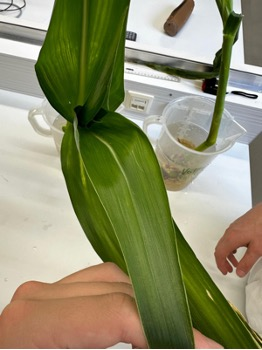
\includegraphics[width=\textwidth]{Vollmedium_.jpg}
				\caption{Vollmedium}
				\label{fig:_voll}
			\end{subfigure}
			\hfill
			\begin{subfigure}[b]{0.31\textwidth}
				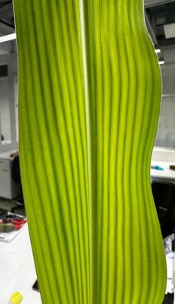
\includegraphics[width=\textwidth]{MinusMg_.jpg}
				\caption{$\ominus$Mg - Medium}
				\label{fig:minus mg_}
			\end{subfigure}
			\hfill
			\begin{subfigure}[b]{0.235\textwidth}
				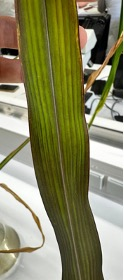
\includegraphics[width=\textwidth]{MinusP_.jpg}
				\caption{$\ominus$P - Medium}
				\label{fig:minus P_}
			\end{subfigure}
			\hfill
			\vspace*{0.8cm}
			\begin{subfigure}[b]{0.25\textwidth}
				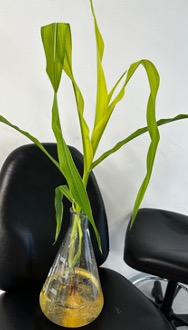
\includegraphics[width=\textwidth]{MinusFe.jpg}
				\caption{$\ominus$Fe - Medium}
				\label{fig:minus Fe}
			\end{subfigure}
			\hfill
			\begin{subfigure}[b]{0.215\textwidth}
				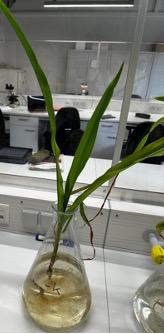
\includegraphics[width=\textwidth]{MinusK.jpg}
				\caption{$\ominus$K - Medium}
				\label{fig:minus K}
			\end{subfigure}
									\hfill
			\begin{subfigure}[b]{0.45\textwidth}
				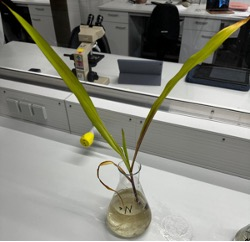
\includegraphics[width=\textwidth]{MinusN.jpg}
				\caption{$\ominus$N - Medium}
				\label{fig:minus N}
				\end{subfigure}
			
			\caption{Bilddokumentation von einzelnen Keimlingspflanzen der Art zea mays in der 5-Blattstadium in unterschiedlichen Nährmedium mit den Fehlenden Micro/Macro-Nährstoffen}
			\label{Mangel}
		\end{figure}
		
		\subsubsection{Wurzelhaare}
		Bei der Untersuchung der Wurzeln von Zea mays im Vollmedium, sowie in einem Medium mit fehlenden Phosphat (P)  und einem weiteren Medium mit fehlenden Eisen (Fe) Verfügbarkeit, sind einige Unterschiede zu erkennen. Während die Wurzeln der Pflanze im Vollmedium keine auffindbaren Wurzelhaare besaß, hatten die Pflanze aus dem Medium ohne P erkennbare Wurzelhaare (siehe Figure \ref{fig:wurzel ohne P}). Bei der Pflanze aus dem Medium ohne Fe konnte man sogar eine noch größere Anzahl an Wurzelhaaren feststellen (siehe Figure \ref{fig:wurzel ohne Fe}). Auch die Länge der Wurzeln und das Verhältnis zum Spross unterschieden sich stark (siehe Table \ref{tab:Verhältnis}). So hatte die Pflanze im Vollmedium ein Spross/Wurzel Verhältnis von ungefähr eins und eine Sprosslänge von 50cm. Verglichen mit den Pflanzen im Medium ohne P eine Sprosslänge von nur 30cm und eine im Verhältnis verlängerte Wurzel hatten (Verhältnis von 0,70). Auch die Pflanze im Medium ohne Fe hat ein verringertes Sprosswachstum im Vergleich zur Vollmedium-Pflanze (37cm). Im Gegensatz zur Pflanze ohne P hat sie jedoch außerdem eine verkürzte Wurzel (21cm), womit das Verhältnis weit über eins liegt (1,76).
		
		\begin{figure}[H]
			\centering
			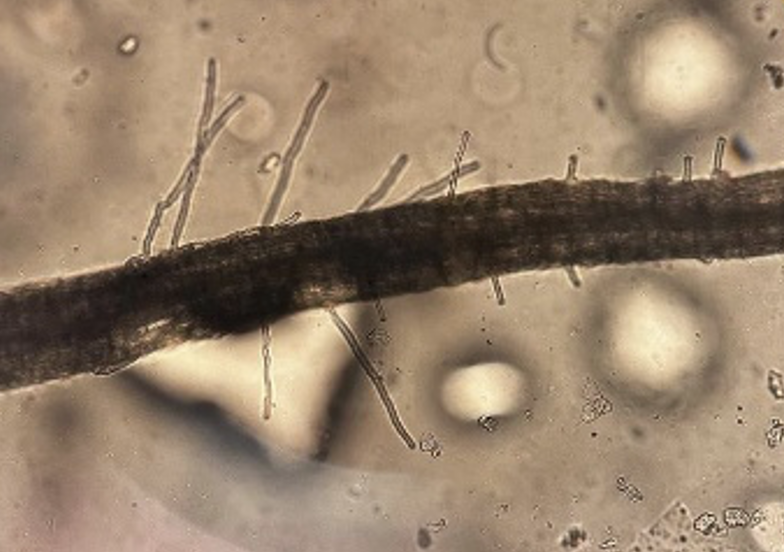
\includegraphics[scale=0.5]{P_minuswurzel}
			\caption{40-fache Vergrößerung der Wurzel einer Zea Mays Pflanze welches in einem Nährmedium ohne Phosphor kultiviert wurde. Sichtbar sind mehrere Wurzelhaare mit unterschiedlichen Längen.}
			\label{fig:wurzel ohne P}
		\end{figure}
		
		
		\begin{figure}[H]
			\centering
			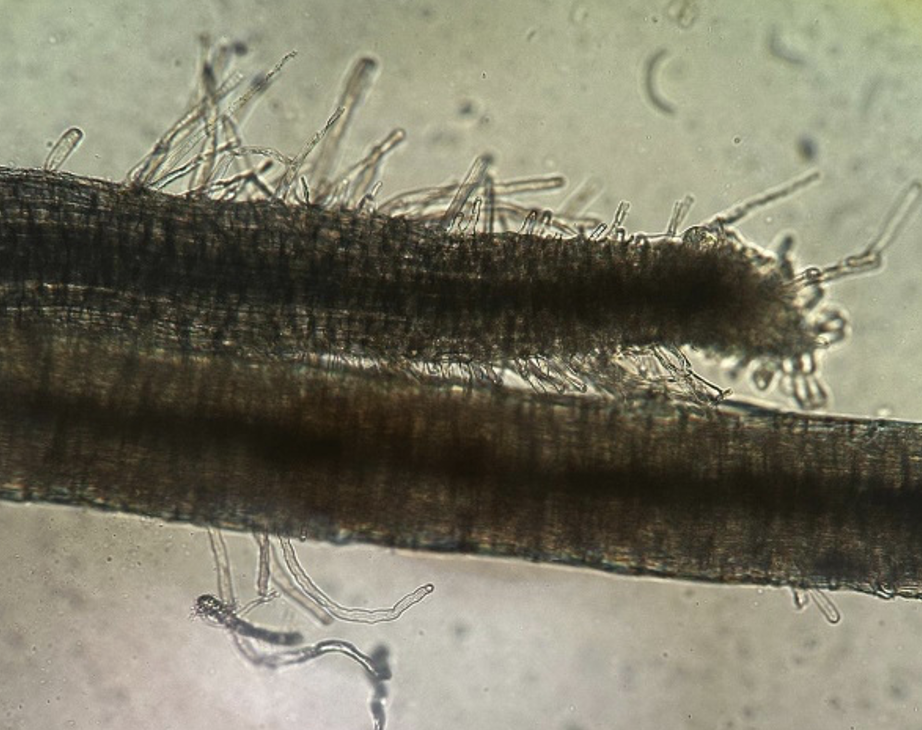
\includegraphics[scale=0.5]{Fe_minus}
			\caption{40-fache Vergrößerung der Wurzel einer Zea Mays Pflanze welches in einem Nährmedium ohne Eisen kultiviert wurde. Sichtbar sind eine große Anzahl an Wurzelhaaren an der Wurzelspitze der oberen Wurzel.}
			\label{fig:wurzel ohne Fe}
		\end{figure}
		
		
		\subsection{Stickstoffaufnahme der Sonnblumenkeimlinge}
		
			\begin{figure}[H]
				\centering
				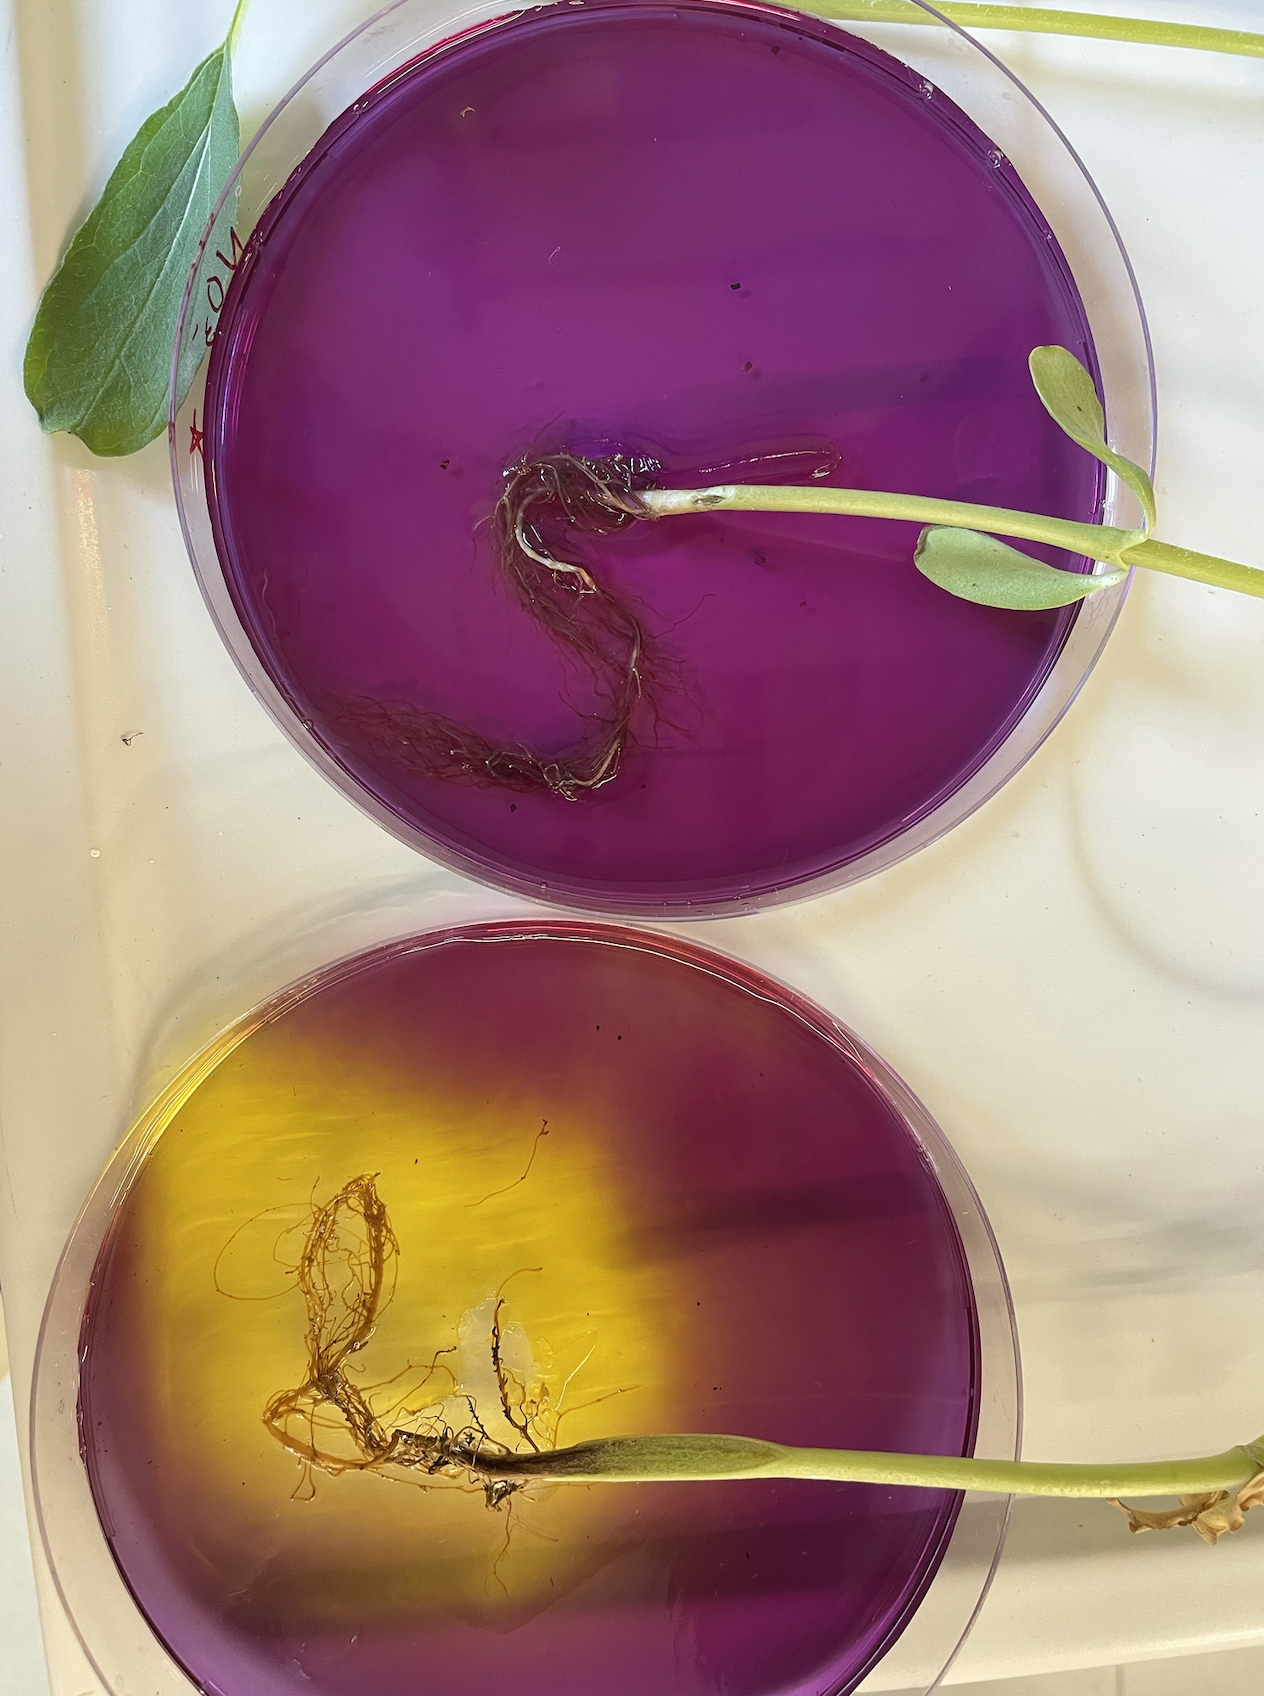
\includegraphics[angle = 90, scale=0.3]{Stickstoffaufnahme.png}
				\caption{3 Wochen altes Sonnenblumenpflanze mit verschiedene Stickstoffaufnahmemethode (links nimmt die Pflanze Nitrat- und rechts Ammonium-Ionen auf)in Bromkresolpurpur-Agar. Die Pflanze wurde für 24h in dem Medium inkubiert.}
				\label{fig:stickstoffaufnahme}
			\end{figure}
			
		Nach circa einem Tag verfärbte sich das Medium der Ammonium-Pflanze an dem Wurzelbereich gelb, während bei der Nitratpflanze das Medium schwach rot bis keine verfärbung zeigt (siehe Firgure \ref{fig:stickstoffaufnahme}).
	
	\section{Diskussion}
	\subsection{Nährstoffmangel}
	Die Bilder des Vollmediums (Figure \ref{fig:_voll}) dienen als Orientierung und Vergleich zu den Metamorphosen der Keimlinge mit einem bestimmten Mangel.\\
	Bei Magnesiummangel verändert sich das Blatt morpholigisch durch sogenannte Streifenchlorose, welches besonders gut im Figure \ref{fig:minus mg_} erkennen kann. Hierbei sind die Blätter nur im Bereich der Leitbündel dunkelgrün, also enthalten dort größere Mengen an Chlorophyll, dazwischen sind sie auch blasser. Magnesium wird im Phloem, nach dem “source to sink”  Modell transportiert, weshalb besonders ältere Blätter - bei neuen Blätter die Blattspitzen (der älteste Teil der Pflanze) - besonders stark von Chlorose betroffen sind. Die Chlorose wird dadurch ausgelöst, dass Magnesium das zentrale Atom im Poryphrinring, dem aktiven Zentrum von Chlorophyll ist. Die Streifenchlorose, also die Konzentrierung von Chlorophyll nahe der Leitbündel, wird durch den “source to sink” Transport bedingt. Hinzukommt ein vermindertes Sprosswachstum, welches sich in den Messwerten widerspiegelt. Dies ist einerseits durch die verringerte Photosynthese, durch weniger Chlorophyll bedingt und dadurch, dass Magnesium ein Cofaktor für sämtliche Proteine ist, was zu weiteren Schwächeerscheinungen bei Mangel, bzw. Fehlen führt. \\
	  \\
	Die Morphologie einer Keimlingspflanze in einem Medium ohne Phosphor(siehe Figure \ref{minus P_}) wird einerseits charakterisiert durch eine Streifenchlorose (vergleich Figure \ref{fig:minus mg_}) und eine unregelmäßige Grünfärbung der Blätter. Außerdem kann eine Rotfärbung beobachtet werden. Anhand der Messwerte kann man eine starke Verringerung des Sprosswachstums (weniger als halb so groß wie beim Vollmedium) und eine Verringerung des Wurzelwachstums. Dies ist bedingt durch eine Hemmung der Meristemaktivität und des Wachstums, da Phosphor entscheidend ist für die Zellteilung. Verringertes Wachstum führt wiederum zu verringerter Photosyntheseaktivität, da weniger Blattfläche verfügbar ist, was sich daraufhin selbst bewirkt. Man muss natürlich die entscheidende Rolle von Phosphor in ATP beachten, dem universellen Energieträger, weshalb eine Mangelernährung zu verminderter Energieübertragung führt und die Stoffwechselrate dämmt.\\
	Die Rotfärbung kann durch eine Anthocyanbildung, aus dem Phenylpropanoid-Stoffwechsel, erklärt werden - eine Antwort auf den zellulären Stress des Phosphormangels. Zudem können Anthocyane, bei Phosphormangel entstehende, reaktive Sauerstoffspezies neutralisieren und dadurch die Pflanze vor oxidativem Stress schützen. Letztlich können Anthocyane überschüssige Lichtenergie aufnehmen, welche von fehlenden Chlorophyllen nicht aufgenommen werden kann.\\
	Die Wurzeln eines Keimlings mit Phosphormangel sind zudem stark verzweigt und bilden, im Vergleich zu der im Vollmedium, deutlich mehr Wurzelhaare (siehe Figure \ref{fig:wurzel ohne P}).\\
	\\
	Auch bei EIsenmangel zeigt die Pflanze Streifenchlorose (Vergleich Figure \ref{fig:minus mg_} und \ref{fig:minus P_}). Bei Eisenmangel hingegen ist diese jedoch stärker bei jüngeren Blättern zu beobachten - diese erscheinen, wie es im Bild zu erkennen ist, welk und blass, da noch genug Eisen in dem Samen verfügbar ist, um die ersten Blätter zu versorgen.
	Dies liegt einerseits daran, dass Eisen ein Cofaktor für die Proteinklasse der Cytochrome ist, welche in den Mitochondrien bei der Zellatmung und Energieproduktion aktiv ist, welche besonders wichtig für junge und sich schnell teilende sind. \\
	Andererseits kommt hinzu, dass Eisen im Boden vorwiegend in schwerlöslichen Eisen(III)-oxiden und Hydroxiden vorliegt. Um toxische Effekte durch freie Eisenionen zu vermeiden, werden stabile Komplexe mit Chelatoren und Phytosiderophoren gebildet, welche jedoch nur schwer transportiert im Phloem werden können. Daher wird Eisen, in der Regel, in den Geweben eingelagert in welchen es aufgenommen wird und bleibt dort. \\
	Die Wurzeln eines Keimlings mit Phosphormangel sind zudem stärker verzweigt und bilden, im Vergleich zu der im Vollmedium, deutlich mehr Seitenwurzeln.\\
	\\
	Bei fehlenden Kalium wird der Wachstum gehemmt, Die Blätter verwelken und können nekrotisch werden, besonders an den Blattspitzen. \\
	Dies kann durch die vielfältigen Funktionen von Kalium in der Pflanze erklärt werden. Darunter ist die zentrale Rolle bei der Regulierung des Turgordrucks, da es bei der Aktivität der Stomata beteiligt ist, welche den Gasaustausch und den Wasserverlust durch Transpiration kontrollieren. Zudem ist Kalium relevant für die Aufrechterhaltung des Membranpotentials, unter anderem an den Chloroplasten. Hierbei ist das Membranpotential notwendig für die Erzeugung von ATP. Außerdem ist Kalium ein Cofaktor für mehr als 60 Enzyme, welche unter anderem in der Proteinsynthese und der Zuckersynthese aus Stärke relevant sind. Das Sprosswachstum ist aus diesen zahlreichen Gründen, aufgrund mangelnder Energie stark verringert. Dies kann durch das Verhältnis Sproos und Wurzel auch beobachtet werden, da diese weit unter 1 beträgt (siehe Table \refeq{tab:Verhältnis})\\
	\\
	Die Morphologie wird charakterisiert durch Chlorose, Wachstumshemmungen, Verwelkung der Blätter, Anthrocyanfärbung (siehe Figure \ref{fig:minus P_}) und Nekrosen, besonders an den Blattspitzen. Man kann außerdem eine extrem starke Verlängerung der Wurzeln, insbesondere der Hauptwurzel, beobachten. In unseren Messungen ist die Wurzellänge mehr als doppelt so groß wie im Vollmedium (siehe Table \refeq{tab:Verhältnis}). Der Spross ist, ähnlich wie bei Kaliummangel, extrem verkürzt, es sind nur zwei Blätter zu beobachten.\\
	Das Verhältnis von Spross zu Wurzel spricht für sich selbst und ist das drastischste Resultat in unseren Messungen.\\
	Dies kann man darauf zurückführen, dass Stickstoff in sämtlichen, für das Überleben notwendigen Verbindungen vorkommt: Aminosäuren, Amiden, Nukleinsäuren, Coenzymen etc. Dadurch ist die Proteinsynthese, Energieübertragung und daher das Wachstum extrem eingeschränkt. Wie bereits behandelt, führt vermindertes Wachstum im Umkehrschluss zu verminderter Nährstoffaufnahme, Energieübertragung, Photosynthese und deshalb ultimativ wieder zu vermindertem Wachstum. 
	
	
	
	\subsubsection{Wurzelhaare}
	Wie im Ergebnisteil beschrieben konnte eine ganze klare Veränderung der Wurzelmorphologie, sowie des Spross- und Wurzelwachstums, abhängig vom vorhanden sein und nicht-vorhanden sein unterschiedlicher Mirko- bzw. Makronährstoffe erkannt werden. Die unterschiedlichen morphologischen Anpassungen lassen sich durch verschiedene Prozesse, die durch Nährstoffmangel ausgelöst werden, erklären. Die Anpassungen der Wurzelmorphologie an den Mangel eines oder mehrerer Nährstoffe ist nur ein Teil der Pflanzen-umfassenden Anpassung, die in Teilen bereits beschrieben wurde. Da jedoch die Wurzel das Organ ist, welches für die Aufnahme der Mikro- und Makronährstoffe zuständig ist, kann besonders hier die Veränderung ein wichtiger Indikator für einen Nährstoffmangel sein.\\
	Da P und P-haltige Verbindungen eine schlechte Löslichkeit in Wasser haben, kann P nicht einfach mit dem Wassersog durch die Erde zur Pflanze hin transportiert werden. Vor allem bei geringer Verfügbarkeit von P im Boden ist es für die Pflanze wichtig nicht nur eine effektive P-Aufnahme zu gewährleisten sondern auch durch ständiges Wachstum der Wurzeln, neue, ungenutzte Erde zu erschließen\cite{Taiz}. P liegt im Boden häufig in anorganischen Metall-Verbindungen mit positiv geladenen Ionen (z.B. Calcium-Ionen, Fe-Ionen) vor. Um eine bessere Aufnahme zu erzielen, säuern manche Pflanzen den Boden um die Wurzeln (Rhizosphäre) an.  Bei der Aufnahme von weiter entferntem P hilft die Symbiose mit Mykorrhiza-Pilzen, die mit ihren Hyphen weiter in die Erde wachsen und die Pflanze mit weiteren Nährstoffen versorgen können\cite{Taiz}. Als Reaktion auf geringe P Verfügbarkeit wird nicht nur das Wurzelwachstum angeregt, sondern auch das Wachstum von Wurzelhaaren. So konnte bei Arabidopsis thaliana eine fünffach höhere Wurzelhaardichte und längere Wurzelhaare bei geringer P-Verfügbarkeit festgestellt werden\cite{Schaaf;}. Wurzelhaare spielen demnach eine wichtige Rolle in der Aufnahme von P, da sie die Oberfläche der Wurzeln vergrößern und weiter in die Erde reichen.\\
	Im Boden ist Fe vor allem in Form von unlöslichem Fe(III) vorhanden. Gerade in Regionen mit kalkhaltigem Boden, ist es für Pflanzen schwer Fe aus dem Boden zu lösen. So sind schätzungsweise 30$\%$ der weltweit landwirtschaftliche genutzten Flächen zu kalkhaltig für eine optimales Pflanzenwachstum\cite{Barker}. Z. mays nutzt zur Aufnahme von Fe aus der Erde eine spezielle Klasse von Chelaten. Diese sogenannten Phytosidophore (PS) sind hochaffine Komplexbildner. PS bestehen aus Aminosäuren, die typischerweise nicht in Proteinen gefunden werden. Die PS werden von den Wurzelzellen in die Erde abgegeben und bilden dort mit Fe(III) stabile Komplexe. Anschließend können die PS-Fe(III)-Komplexe durch ein spezielles PS Transportsystem aufgenommen werde\cite{Taiz}. Die Aufnahme in die Wurzelepidermiszellen erfolgt über den hochaffinen ZmYS1 Transporter in der Zellmembran\cite{Schaaf;}. Die Bildung dieser Transporter wird durch Fe-Mangel induziert und gleichzeitig werden mehr PS in den Boden abgegeben. Einmal in die Pflanze aufgenommen wird der Komplex durch das Xylem in der Pflanze verteilt\cite{Taiz}.  Fe-Mangel führt außerdem auch zur Bildung von verzweigten Wurzelhaaren sowie einer vergrößerten Wurzelhaarzone. Diese Veränderung dient der Vergrößerung der Oberfläche und damit auch dem Kontakt mit mehr Fe-Molekülen. Dabei kann man auf Figure \ref{fig:wurzel ohne Fe} (Fe Mangel), nicht erkennen, ob es sich um verzweigte Wurzelhaare handelt. 
	
	\subsection{Stickstoffaufnahme}
	Damit die Pflanze Stickstoff in Form von Ammonium aufnehmen kann, muss die Pflanze den umliegende Ammoniak ein Proton anbieten. Ammonium-Ionen-Aufnahme ist anders als Ammoniak nicht toxisch. Es gibt einige Strategien die die Pflanze hat, um Ammonium aufnehmen zu können, eins davon ist eine Protonen/Ammonium-Symport-Mechanismus und das andere ist ein Protonengradienten außerhalb der Wurzelmembran aufzubauen. Bei beiden methoden wird die umliegende Rhizosphäre angesäurert.\\
	Das kann kann in Figure \ref{fig:stickstoffaufnahme} rechts gut sehen. Da Bromkresolpurpur bei saueren/niedriegen pH-Wert zu Gelb umschlägt.\\
	\\
	Bei der Aufnahme von Nitrat muss die Pflanze gleichzeitig PRotonen mithilfe einen Protonen-Co-Transporter aufnehmen, wodurch die Umgebung alkalischer wird. Dies konnte leider nicht nach 24 h beobachtet werden.\\
	Der Indikator sollte sich bei hohen pH-Wert zu violett verfärben. \\
	Für eine Wiederholung des Versuches kann die Inkubationszeit auf mehr als einem Tag verlängert werden oder einen anderen Indikator verwendet werden, wo der alkalischen Bereich deutlich von den neutralen Bereich farblich unterscheidet.
	
	\addcontentsline{toc}{section}{References}
	\bibliographystyle{plainurl}
	\nocite{*}
	\bibliography{Literatur}
	\newpage
	
	
\end{document}